\setcounter{dang}{0}
\section{HÀM SỐ MŨ, HÀM SỐ logarit}
\subsection{Lý thuyết cần nhớ}
\subsubsection{Hàm số mũ}
\begin{itemize}
	\item [\iconMT] \indam{Dạng:} $y=a^x$, trong đó $0<a \ne 1$.
	\begin{itemize}
		\item [\ding{172}] Tập xác định của hàm số $y=a^x$ là $\mathbb{R}$;
		\item [\ding{172}] Tập giá trị của hàm số $y=a^x$ là $(0;+\infty)$.
	\end{itemize}

	\item [\iconMT] \indam{Đồ thị hàm số $y=a^x$:}
	\begin{listEX}[1]
		\item [\ding{172}]\,\, Khi $a>1$ thì hàm số đồng biến trên $\mathbb{R}$.
		\item [\ding{173}]\,\, Khi $0<a<1$ thì hàm số nghịch biến trên $\mathbb{R}$.
		\item [\ding{174}]\,\, Đồ thị luôn qua $(0;1)$ và luôn nằm phía trên trục hoành.
		\end{listEX}
		\begin{center}
			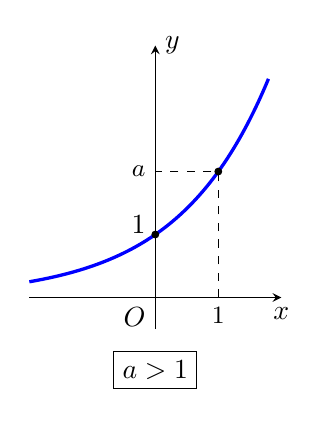
\begin{tikzpicture}[smooth,samples=300,scale=0.8,>=stealth]
	\draw[->] (-2,0)--(2,0) node[below]{$x$};
	\draw[->] (0,-0.5)--(0,4) node[right]{$y$};
	\draw (0,0) node[below left]{$O$};
	\draw[line width=1.2pt,color=blue,domain=-2:1.8] plot(\x,{2^(\x)});
	\draw[fill=black] (0,1) circle(1.5pt) (1,2) circle(1.5pt);
	\draw[dashed] (1,0)node[below]{\small$1$}--(1,2)--(0,2)node[left]{\small$a$};
	\node[below] at (0,-0.7) {\fbox{$a>1$}};
	\node[left] at (0,1.15) {$1$};
	\end{tikzpicture}	
	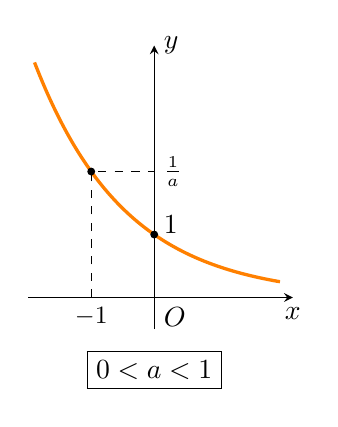
\begin{tikzpicture}[smooth,samples=300,scale=0.8,>=stealth]
	\draw[->] (-2,0)--(2.2,0) node[below]{$x$};
	\draw[->] (0,-0.5)--(0,4) node[right]{$y$};
	\draw (0,0) node[below right]{$O$};
	\draw[line width=1.2pt,color=orange,domain=-1.9:2] plot(\x,{0.5^(\x)});
	\draw[fill=black] (0,1) circle(1.5pt) (-1,2) circle(1.5pt);
	\draw[dashed] (-1,0)node[below]{\small$-1$}--(-1,2)--(0,2)node[right]{\small$\frac{1}{a}$};
	\node[below] at (0,-0.7) {\fbox{$0<a<1$}};
	\node[right] at (0,1.15) {$1$};
	\end{tikzpicture}
		\end{center}	
\end{itemize}
\subsubsection{Hàm số logarit}
\begin{itemize}
	\item [\iconMT] \indam{Dạng:} $y=\log_ax$, trong đó $0<a \ne 1$ và $x>0$.
	\begin{itemize}
		\item [\ding{172}] Tập xác định của hàm số $y=\log_ax$ là $(0;+\infty)$ ;
		\item [\ding{172}] Tập giá trị của hàm số $y=\log_ax$ là $\mathbb{R}$ .
	\end{itemize}
	\item [\iconMT] \indam{Đồ thị hàm số $y=\log_ax$:}
	\begin{listEX}[1]
		\item [\ding{172}]\,\, Khi $a>1$ thì hàm số đồng biến trên $(0; +\infty)$ 
		\item [\ding{173}]\,\, Khi $0<a<1$ thì hàm số nghịch biến trên $(0; +\infty)$ .
		\item [\ding{174}]\,\, Đồ thị luôn qua $(1;0)$ và luôn nằm bên phải trục tung.
	\end{listEX}
	\begin{center}
		\begin{tikzpicture}[smooth,samples=300,scale=0.8,>=stealth]
	\draw[->] (-1,0)--(4,0) node[below]{$x$};
	\draw[->] (0,-2.5)--(0,2) node[right]{$y$};
	\draw (0,0) node[below left]{$O$};
	\draw[line width=0.8pt,color=violet,domain=0.2:3.2]plot(\x,{ln((\x))/ln(2)});
	\draw[fill=black] (1,0) circle(1.5pt) (2,1) circle(1.5pt);
	\draw[dashed] (2,0)node[below]{\small$a$}--(2,1)--(0,1)node[left]{\small$1$};
	\node[below] at (1,-2.6) {\fbox{$a>1$}};
	\node[below] at (1.1,0) {\small$1$};
	\end{tikzpicture}
	\begin{tikzpicture}[smooth,samples=300,scale=0.8,>=stealth]
	\draw[->] (-1,0)--(4,0) node[below]{$x$};
	\draw[->] (0,-2)--(0,2.5) node[left]{$y$};
	\draw (0,0) node[below left]{$O$};
	\draw[line width=0.8pt,color=violet,domain=0.2:3.2]plot(\x,{ln((\x))/ln(0.5)});
	\draw[fill=black] (1,0) circle(1.5pt) (2,-1) circle(1.5pt);
	\draw[dashed] (2,0)node[above]{\small$\dfrac{1}{a}$}--(2,-1)--(0,-1)node[left]{\small$-1$};
	\node[below] at (1,-2.2) {\fbox{$0<a<1$}};
	\node[above] at (1.1,0) {\small$1$};
	\end{tikzpicture}
	\end{center}
	
\end{itemize}
\subsection{Các dạng toán thường gặp}
\begin{dang}{Tìm tập xác định}
	\begin{itemize}
		\item [\iconMT] Đối với hàm số $y=a^{u(x)}$: Ta chỉ cần tìm điều kiện để $u(x)$ có nghĩa.
		\item [\iconMT]  Đối với hàm số $y=\log_a{u(x)}$: Ta tìm điều kiện để $u(x)>0$.\\		
		Với hàm số $y=\log_ab^{2n}$, ta chỉ cần điều kiện $b \ne 0$.
	\end{itemize}
\end{dang}

\begin{vd}
	Tìm tập xác định $\mathscr{D}$  của các hàm số sau:
	\begin{enumEX}[a)]{3}
		\item $y=\log_{2}x $;
		\item  $y=\log_3(x-2)$;
		\item  $y=\log_{\frac{1}{3}}(4-2x)$; 
		\item $ y=\log_{3}(x^{2}-x-2) $;
		\item $y=\ln\left(x^2+3x+2\right)$;
		\item $y=\log_5\dfrac{x-3}{x+2}$.
	\end{enumEX}
	\loigiai{
		\begin{enumerate}[a)]
		\item Hàm  số  $y=\log_{2}x $ xác định khi $x>0$.\\
		Do đó tập xác định của hàm số  $\mathscr{D}= (0;+\infty)$.
		\item Điều kiện $x-2>0\Rightarrow x>2$. Tập xác định $\mathscr{D}=(2;+\infty)$.
		\item Hàm số xác định khi và chỉ khi $4-2x>0\Leftrightarrow x<2$.\\
		Vậy tập xác định của hàm số là $\mathscr{D}=(-\infty;2)$.
		\item Điều kiện xác định $ x^{2}-x-2>0\Leftrightarrow x<-1 $ hoặc $ x>2 $. Suy ra $ \mathscr D=(-\infty;-1)\cup (2;+\infty) $.
		\item Hàm số xác định khi $x^2+3x+2>0\Leftrightarrow \hoac{&x<-2\\&x>-1.}$\\
		Vậy tập xác định của hàm số là $(-\infty;-2)\cup(-1;+\infty)$.
		\item Hàm số xác định khi $ \frac{x-3}{x+2}>0 \iff x\in (-\infty;-2)\cup (3;+\infty)$.
	\end{enumerate}}
\end{vd} \dongcham{10}

\begin{vd}%[2D2Y4-1]%
	Tìm tập xác định $\mathscr{D}$ của các hàm số sau:
	\begin{enumEX}[a)]{3}
		\item $y = \log_{3}x^2 $;
		\item $y = \log_{3}\left(4-x^2 \right)^4$;
		\item $y = \dfrac{1}{\log_{3}x}$;
		\item $y = \dfrac{1}{\log_{3}(x-1)}$;
		\item $y = \log\left|\sin x\right|$;
		\item $y = \ln\left(1- \cos x \right)$.
	\end{enumEX}
	\loigiai{
	}
\end{vd} \dongcham{12}

\begin{dang}{Đồ thị hàm số}
	Để vẽ đồ thị hàm mũ $y=a^x$ hoặc hàm logarit $y=\log_a x$, ta làm như sau:
	\begin{listEX}[1]
		\item [\ding{172}] Lập bảng giá trị của hàm số cần vẽ;
		\item [\ding{173}] Căn cứ vào cơ số và hình dáng đồ thị, ta vẽ đường cong qua các điểm đã cho.
	\end{listEX}
\end{dang}

\begin{vd}%[1K6BJ-2]
	Vẽ đồ thị của các hàm số mũ sau:
	\begin{listEX}[4]
		\item $y=2^x$;
		\item  $y=(\sqrt{3})^x$;
		\item $y=\mathrm{e}^x$;
		\item  $y=\left(\dfrac{1}{4}\right)^x$.	
		\item $y=\log_2 x$;
		\item  $y=\log_{\sqrt{3}}x$;
		\item $y=\ln x$;
		\item  $y=\log_{\frac{2}{3}}x$.	
	\end{listEX}
	\loigiai{
	}
\end{vd} \dongcham{32}

\begin{vd}
	\immini{
		Cho số thực $ a $ dương, khác $ 1 $. Biết rằng bất kỳ đường thẳng nào song song với trục $ Ox $ mà cắt các đường $ y=4^{x} $, $ y=a^{x} $, trục tung lần lượt tại $ M $, $ N $, $ A $ thì $ AN=2AM $ (hình vẽ bên). Tính $a$.
	}{
		\begin{tikzpicture}[line join=round, line cap=round,>=stealth]
			\tikzset{label style/.style={font=\footnotesize}}
			\pgfmathsetmacro\h{1}
			\pgfmathsetmacro\xmin{-2.2*\h}
			\pgfmathsetmacro\xmax{2.5*\h}
			\pgfmathsetmacro\ymin{-0.5*\h}
			\pgfmathsetmacro\ymax{3.5*\h}
			\clip(\xmin-0.01,\ymin-0.01)rectangle(\xmax+0.01,\ymax+0.01);
			\def\hamsoa{4^(\x)}
			\def\hamsob{(1/2)^(\x)}
			\draw[->](\xmin,0)--(\xmax,0)node[below left]{$x$};
			\draw[->](0,\ymin)--(0,\ymax)node[below left]{$y$};
			\draw(0,0)node[below left]{\fontsize{12pt}{1pt}\selectfont O};
			\draw[samples=100,domain=\xmin+0.01:\xmax-0.01,smooth,variable=\x]plot(\x,{\hamsoa});
			\draw[samples=100,domain=\xmin+0.01:\xmax-0.01,smooth,variable=\x]plot(\x,{\hamsob});
			\node[below left,xshift=1.2cm]at(1,3){$y=4^{x}$};
			\node[above right]at(1,0.5){$y=a^{x}$};
			\tkzDefPoints{-1/2/N,0/2/A,0.5/2/M}
			\tkzDrawPoints[fill=black](A,M,N)
			\draw (N)--(M);
			\tkzLabelPoints[above left](A)
			\tkzLabelPoints[below left](N)
			\tkzLabelPoints[below right](M)
		\end{tikzpicture}
	}
	\loigiai{
		Giả sử $ M $, $ N $ có hoành độ lần lượt là $ m $, $ n $. Theo đề bài ta có
		\[
		-n=2m\text{ và }a^{n}=4^{m}\Rightarrow a^{-2m}=4^{m}\Rightarrow \left(4a^{2}\right)^{m}=1\Rightarrow 4a^{2}=1\Rightarrow a=\dfrac{1}{2}.
		\]
	}
\end{vd} \dongcham{7}

\begin{dang}{Vận dụng. Thực tiễn}
	
\end{dang}

\begin{vd}
	Đồ thị Hình bên dưới cho thấy số lượng hươu cao cổ trên thế giới suy giảm nghiêm trọng trong 30 năm qua (từ năm 1985 đến 2015) (nguồn: https://tuoitre.vn/huou-cao-co-sap-vao-danhsach-loai-gap-nguy-hiem-20190428162017473.htm). 
	\begin{center}
		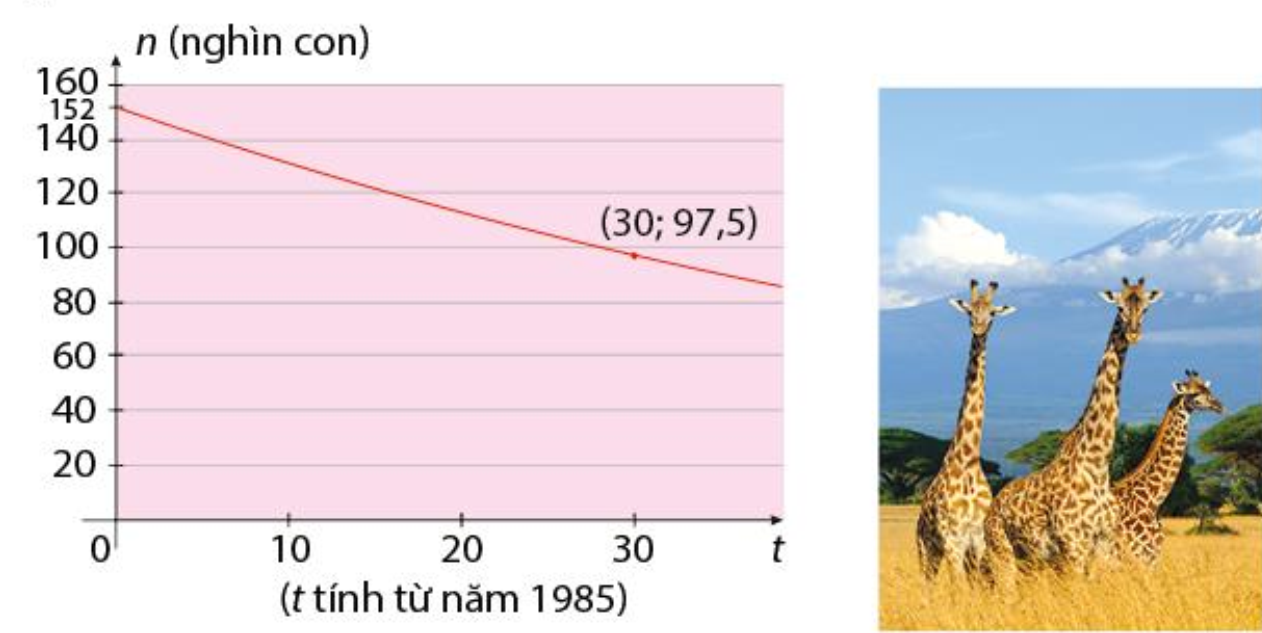
\includegraphics[scale=0.35]{data/11KNTT/data6/h1.png}
	\end{center}
	Giả sử rằng số lượng hươu ở đây giảm theo hàm số $n(t)=C \cdot a^t$.
	\begin{enumEX}[a)]{1}
		\item Tìm số lượng hươu vào năm 1985.
		\item Tìm hàm số biểu diễn số lượng hươu sau $t$ năm kể từ năm 1985.
		\item Dự đoán số lượng hươu vào năm 2025.
	\end{enumEX}
	\loigiai{
		\begin{enumerate}[a)]
			\item
			\item
			\item
	\end{enumerate}}
\end{vd} \dongcham{6}

 \begin{vd}%[1D4K3-4]
	Các nhà khoa học xác định được chu kì bán rã của ${ }_6^{14} \mathrm{C}$ là $5730$ năm, tức là sau 5730 năm thì số nguyên tử ${ }_6^{14} \mathrm{C}$ giảm đi một nửa.
	\begin{listEX}[1]
		\item Gọi $m_0$ là khối lượng của ${ }_6^{14} \mathrm{C}$ tại thời điểm $t=0$. Viết công thức tính khối lượng $m(t)$ của ${ }_6^{14} \mathrm{C}$ tại thời điểm $t$ (năm).
		\item Một cây còn sống có lượng ${ }_6^{14} \mathrm{C}$ trong cây được duy trì không đổi. Nhưng nếu cây chết thì lượng ${ }_6^{14} \mathrm{C}$ trong cây phân rã theo chu ki bán rã của nó. Các nhà khảo cồ đã tìm thấy một mẫu gỗ cổ được xác định chết cách đây 2000 năm. Tính tỉ lệ phần trăm lượng ${ }_6^{14} \mathrm{C}$ còn lại trong mẫu gỗ cổ đó so với lúc còn sinh trường (làm tròn kết quả đến hàng phần mười).
	\end{listEX}
	\loigiai{
		\begin{listEX}[1]
			\item Ta có $m(t)=m_0 \cdot\left(\dfrac{1}{2}\right)^{\dfrac{t}{5730}}$.
			\item Tỉ lệ phần trăm lượng ${ }_6^{14} \mathrm{C}$ còn lại trong mẫu gỗ cổ đó so với lúc còn sinh trường là
			$$
			\dfrac{m(2000)}{m_0} \cdot 100 \%=\left(\dfrac{1}{2}\right)^{\tfrac{2000}{5730}} \cdot 100 \% \approx 78,5 \% \text {. }
			$$
		\end{listEX}		
	}
\end{vd} \dongcham{10}

\subsection{Bài tập tự luyện}

\begin{bt}%[1D4B3-2]
	Lập bảng biến thiên và vẽ đồ thị các hàm số
	\begin{listEX}[4]
		\item $y=\left(\sqrt{2}\right)^x$;
		\item $y=\left(\dfrac{1}{\sqrt{2}}\right)^x$;
		\item $y=\log_{\sqrt{3}}x$;
		\item $y=-\log_{2}x$. 
	\end{listEX}
	\loigiai{
		\begin{listEX}[1]
			\item $y=\left(\sqrt{2}\right)^x$\\
			Vì hàm số $y=\left(\sqrt{2}\right)^x$ có cơ số $\sqrt{2}>1$ nên ta có bảng biến thiên sau
			\begin{center}
				\begin{tikzpicture}
					\tkzTabInit[nocadre=false,lgt=3,espcl=2,deltacl=0.6]
					{$x$ /0.6,$y=\left(\sqrt{2}\right)^x$/2}
					{$-\infty$,$0$,$+\infty$}
					\draw 
					(N12) node[above] (A) {$-\infty$}
					($(N21)!.3!(N22)$) node(B) {$1$}
					(N31) node[below] (C) {$+\infty$};
					\draw[-stealth] (A)--(C);
				\end{tikzpicture}
			\end{center} 
			Ta có đồ thị hàm số như sau
			\begin{center}
				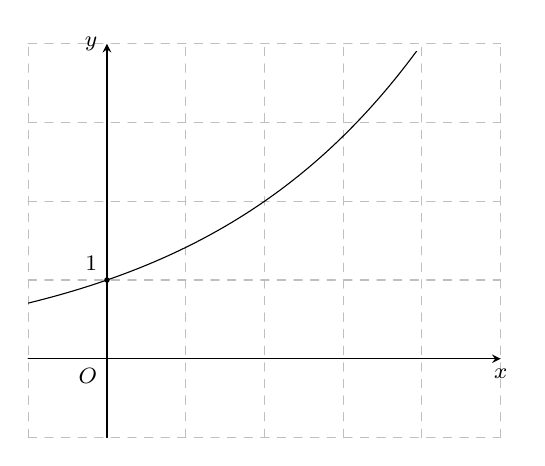
\begin{tikzpicture}[scale=1,>=stealth, font=\footnotesize, line join=round, line cap=round]
					\def\xmin{-1} \def\xmax{5}  \def\ymin{-1}\def\ymax{4}
					\draw[color=gray!50,dashed] (\xmin,\ymin) grid (\xmax,\ymax);
					\draw[->] (\xmin,0)--(\xmax,0) node [below]{$x$};
					\draw[->] (0,\ymin)--(0,\ymax) node [left]{$y$};
					\node at (0,0) [below left]{$O$};
					\fill[black] (0,1) circle (1pt);
					\node at (0,1)[above left]{$1$};
					\clip (-1,-1) rectangle (\xmax-0.1,\ymax-0.1);
					\draw[domain=-1:5,smooth,samples=300] plot(\x,{1.414213562^(\x)});		
				\end{tikzpicture}
			\end{center}				
			\item $y=\left(\dfrac{1}{\sqrt{2}}\right)^x$
			Vì hàm số $y=\left(\dfrac{1}{\sqrt{2}}\right)^x$ có cơ số\\ $\dfrac{1}{\sqrt{2}}<1$ nên ta có bảng biến thiên sau
			\begin{center}
				\begin{tikzpicture}
					\tkzTabInit[nocadre=false,lgt=3,espcl=2,deltacl=0.6]
					{$x$ /0.6,$y=\left(\dfrac{1}{\sqrt{2}}\right)^x$/2}
					{$-\infty$,$0$,$+\infty$}
					\draw 
					(N11) node[below] (A) {$+\infty$}
					($(N21)!.3!(N22)$) node(B) {$1$}
					(N32) node[above] (C) {$-\infty$};
					\draw[-stealth] (A)--(C);
				\end{tikzpicture}
			\end{center} 
			Ta có đồ thị hàm số như sau
			\begin{center}
				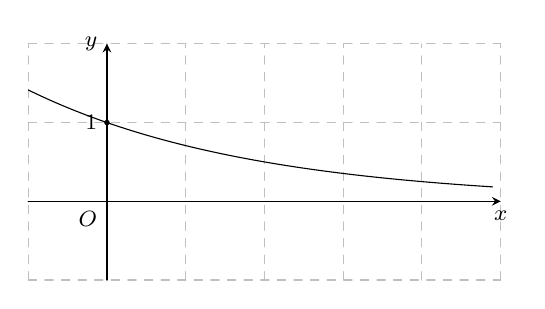
\begin{tikzpicture}[scale=1,>=stealth, font=\footnotesize, line join=round, line cap=round]
					\def\xmin{-1} \def\xmax{5}  \def\ymin{-1}\def\ymax{2}
					\draw[color=gray!50,dashed] (\xmin,\ymin) grid (\xmax,\ymax);
					\draw[->] (\xmin,0)--(\xmax,0) node [below]{$x$};
					\draw[->] (0,\ymin)--(0,\ymax) node [left]{$y$};
					\node at (0,0) [below left]{$O$};
					\fill[black] (0,1) circle (1pt);
					\node at (0,1)[left]{$1$};
					\clip (-1,-1) rectangle (\xmax-0.1,\ymax-0.1);
					\draw[domain=-1:5,smooth,samples=300] plot(\x,{0.7071067812^(\x)});		
				\end{tikzpicture}
			\end{center}				
			\item $y=\log_{\sqrt{3}}x$\\
			Vì hàm số $y=\log_{\sqrt{3}}x$ có cơ số $\sqrt{3}>1$ nên ta có bảng biến thiên sau
			\begin{center}
				\begin{tikzpicture}
					\tkzTabInit[nocadre=false,lgt=3,espcl=2,deltacl=0.6]
					{$x$ /0.6,$y=\log_{\sqrt{3}}x$/2}
					{$0$,$1$,$+\infty$}
					\draw 
					(N12) node[above] (A) {$-\infty$}
					($(N21)!.3!(N22)$) node(B) {$0$}
					(N31) node[below] (C) {$+\infty$};
					\draw[-stealth] (A)--(C);
				\end{tikzpicture}
			\end{center} 
			Ta có đồ thị hàm số như sau
			\begin{center}
				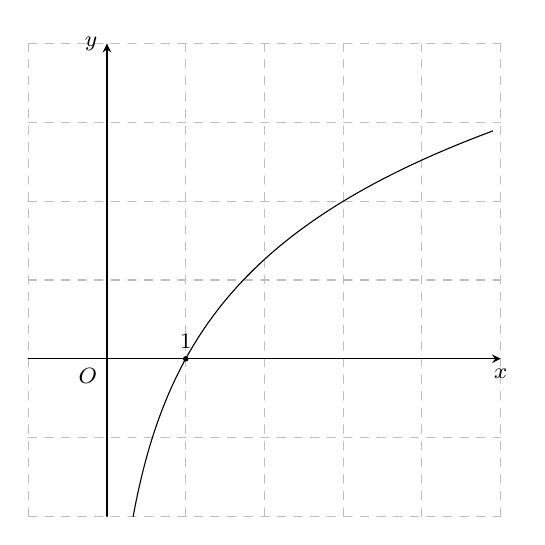
\begin{tikzpicture}[scale=1,>=stealth, font=\footnotesize, line join=round, line cap=round]
					\def\xmin{-1} \def\xmax{5}  \def\ymin{-2}\def\ymax{4}
					\draw[color=gray!50,dashed] (\xmin,\ymin) grid (\xmax,\ymax);
					\draw[->] (\xmin,0)--(\xmax,0) node [below]{$x$};
					\draw[->] (0,\ymin)--(0,\ymax) node [left]{$y$};
					\node at (0,0) [below left]{$O$};
					\fill[black] (1,0) circle (1pt);
					\node at (1,0)[above]{$1$};
					\clip (-1,-2) rectangle (\xmax-0.1,\ymax-0.1);
					\draw[smooth,samples=300,domain=0.03:\xmax] plot(\x,{ln(\x)/0.5493061443});
				\end{tikzpicture}
			\end{center}	
			\item $y=-\log_{2}x$.\\
			Vì hàm số $y=\log_{2}x$ có cơ số $2>1$ nên hàm đồng biến. Suy ra hàm $y=-\log_{2}x$ là hàm nghịch biến
			\begin{center}
				\begin{tikzpicture}
					\tkzTabInit[nocadre=false,lgt=3,espcl=2,deltacl=0.6]
					{$x$ /0.6,$y=-\log_{2}x$/2}
					{$0$,$1$,$+\infty$}
					\draw 
					(N11) node[below] (A) {$+\infty$}
					($(N21)!.3!(N22)$) node(B) {$0$}
					(N32) node[above] (C) {$-\infty$};
					\draw[-stealth] (A)--(C);
				\end{tikzpicture}
			\end{center} 
			Ta có đồ thị hàm số như sau
			\begin{center}
				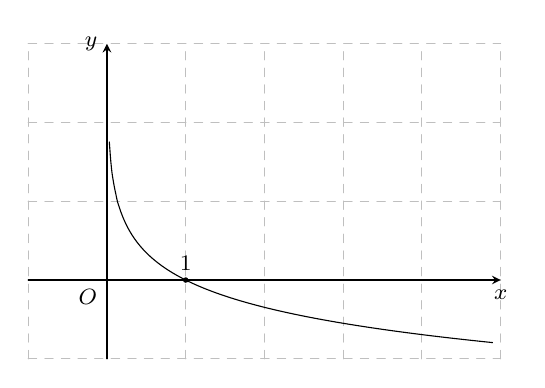
\begin{tikzpicture}[scale=1,>=stealth, font=\footnotesize, line join=round, line cap=round]
					\def\xmin{-1} \def\xmax{5}  \def\ymin{-1}\def\ymax{3}
					\draw[color=gray!50,dashed] (\xmin,\ymin) grid (\xmax,\ymax);
					\draw[->] (\xmin,0)--(\xmax,0) node [below]{$x$};
					\draw[->] (0,\ymin)--(0,\ymax) node [left]{$y$};
					\node at (0,0) [below left]{$O$};
					\fill[black] (1,0) circle (1pt);
					\node at (1,0)[above]{$1$};
					\clip (-1,-1) rectangle (\xmax-0.1,\ymax-0.1);
					\draw[smooth,samples=300,domain=0.03:\xmax] plot(\x,{-ln(\x)/2});
				\end{tikzpicture}
			\end{center}	
		\end{listEX}
	}
\end{bt} \dongcham{17}


\begin{bt}
	So sánh các cặp số sau
	\begin{enumEX}[a)]{2}
		\item $1{,}04^{1{,}7}$ và $1{,}04^2$.
		\item $\left(\dfrac{3}{5}\right)^{-\tfrac{2}{5}}$ và $\left(\dfrac{3}{5}\right)^{-\tfrac{3}{5}}$.
		\item $1{,}2^{0{,}3}$ và $0{,}9^{1{,}8}$.
		\item $\left(\dfrac{1}{3}\right)^{-0{,}4}$ và $3^{-0{,}2}$. 
	\end{enumEX}
	\loigiai{
		\begin{enumerate}
			\item Vì cơ số $1{,}04>1$ và số mũ $1{,}7<2$ nên $1{,}04^{1{,}7}<1{,}04^2$.
			\item Vì cơ số $\dfrac{3}{5}<1$ và số mũ $-\dfrac{2}{5} > -\dfrac{3}{5}$ nên $\left(\dfrac{3}{5}\right)^{-\tfrac{2}{5}} < \left(\dfrac{3}{5}\right)^{-\tfrac{3}{5}}$.
			\item Ta có $\heva{&1{,}2^{0{,}3} > 1^{0{,}3}= 1\\&0{,}9^{1{,}8} < 1^{1{,}8} = 1}$.
			Suy ra $1{,}2^{0{,}3}>0{,}9^{1{,}8}$.
			\item Ta có $\heva{&\left(\dfrac{1}{3}\right)^{-0{,}4} > 1^{-0{,}4} = 1\\& 3^{-0{,}2} < 1^{-0{,}2} = 1}$.
			Suy ra $\left(\dfrac{1}{3}\right)^{-0{,}4}>3^{-0{,}2}$.
		\end{enumerate}
	}
\end{bt} \dongcham{14}

\begin{bt}
	So sánh các cặp số sau
	\begin{enumEX}[a)]{2}
		\item $2 \log _{0{,}6} 5$ và $3 \log _{0{,}6}(2 \sqrt[3]{3})$.
		\item $6 \log _5 2$ và $2 \log _5 6$.
		\item $\dfrac{1}{2} \log _2 121$ và $2 \log _2 2 \sqrt{3}$.
		\item $2 \log _3 7$ và $6 \log _9 4$.
	\end{enumEX}
	\loigiai
	{
		\begin{enumerate}
			\item Ta có $2 \log_{0{,}6} 5=\log_{0{,}6}25$ và $3 \log _{0{,}6}(2 \sqrt[3]{3}) = \log_{0{,}6}24$.\\
			Hàm số $y = \log_{0{,}6}x$ có cơ số $0<0{,}6<1$ nên nghịch biến trên $(0;+\infty)$ và $25>24$ nên $2 \log _{0{,}6} 5<3 \log _{0{,}6}(2 \sqrt[3]{3})$.
			\item Ta có $6 \log _5 2=\log_5 64$ và $2 \log _5 6=\log_5 36$.\\
			Hàm số $y=\log_5x$ có cơ số $5>1$ nên đồng biến trên $(0;+\infty)$ và $64>36$ nên $6 \log _5 2>2 \log _5 6$.
			\item Ta có $\dfrac{1}{2} \log _2 121=\log_2 11$ và $2 \log _2 2 \sqrt{3}=\log_2 12$.\\
			Hàm số $y = \log_2x$ có cơ số $2>1$ nên đồng biến trên $(0;+\infty)$ và $11<12$ nên $\dfrac{1}{2} \log _2 121<2 \log _2 2 \sqrt{3}$.
			\item Ta có $2 \log _3 7=\log_3 49$ và $6 \log _9 4=\log_3 64$.\\
			Hàm số $y = \log_3 x$ có cơ số $3>1$ nên đồng biến trên $(0;+\infty)$ và $ 49<64$ nên $2 \log _3 7<6 \log _9 4$.
		\end{enumerate}
	}
\end{bt} \dongcham{14}

\begin{bt}
	Tìm tập xác định của các hàm số sau:
	\begin{enumEX}[a)]{2}
		\item $y=\log (x-1)$;
		\item $y=\log_{\tfrac{2}{3}}(2020-x)$;
		\item $y=\log(2x-x^2)$;
			\item $y=\log_2\dfrac{3-x}{2 x}$; 
		\item $y=\ln(x-2)^2+\log(x+1)$;
		\item $y=\log_2|x^2-4|$.
	\end{enumEX}
	\loigiai{
		\begin{enumerate}[a)]
			\item Hàm số xác định khi $x-1>0\Leftrightarrow x>1$ hay $x\in (1;+\infty)$.
			\item Hàm số xác định khi và chỉ khi $2020-x>0\Leftrightarrow x<2020$.\\
			Vậy tập xác định của hàm số là $\mathscr{D}=(-\infty;2020)$.
			\item Điều kiện $2x-x^2>0\Leftrightarrow 0<x<2$.\\
			Vậy tập xác định của hàm số là $\mathscr{D}=(0;2)$.
			\item Hàm số đã cho xác định khi $\dfrac{3-x}{2 x}>0\Leftrightarrow x\in(0 ; 3)$.
			\item Hàm số xác định khi và chỉ khi $\heva{&(x-2)^2>0\\&x+1>0}\Leftrightarrow\heva{&x\neq 2\\&x>-1}$.\\
			Vậy $\mathscr{D}=(-1; 2)\cup (2; +\infty)$.
			\item Hàm số xác định khi $|x^2-4|>0\Leftrightarrow x^2-4\ne 0\Leftrightarrow \heva{&x\ne 2\\ &x\ne -2.}$
	\end{enumerate}}
\end{bt} \dongcham{10}

\begin{bt}%[1D4B3-3]
	Dựa vào đồ thị hàm số, cho biết với giá trị nào của $x$ thì đồ thị hàm số $y=\log_{3}x$:
	\begin{listEX}[2]
		\item Nằm phía trên đường thẳng $y=1$;
		\item Nằm phía dưới trục hoành.
	\end{listEX}
	\loigiai{		
		Ta có đồ thị hàm số $y=\log_{3}x$
		\begin{center}
			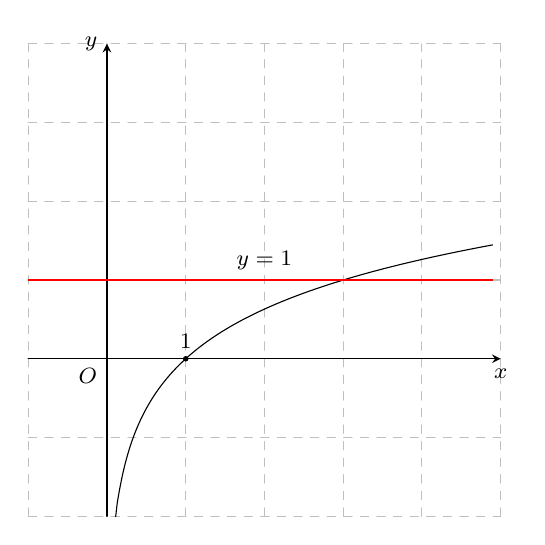
\begin{tikzpicture}[scale=1,>=stealth, font=\footnotesize, line join=round, line cap=round]
				\def\xmin{-1} \def\xmax{5}  \def\ymin{-2}\def\ymax{4}
				\draw[color=gray!50,dashed] (\xmin,\ymin) grid (\xmax,\ymax);
				\draw[->] (\xmin,0)--(\xmax,0) node [below]{$x$};
				\draw[->] (0,\ymin)--(0,\ymax) node [left]{$y$};
				\node at (0,0) [below left]{$O$};
				\fill[black] (1,0) circle (1pt);
				\node at (1,0)[above]{$1$};
				\clip (-1,-2) rectangle (\xmax-0.1,\ymax-0.1);
				\draw[smooth,samples=300,domain=0.03:\xmax] plot(\x,{ln(\x)/ln(3)});
				\draw[red] (-1,1)--(6,1); \node at (2,1)[above]{$y=1$};
			\end{tikzpicture}
		\end{center}	
		\begin{listEX}[1]
			\item Dựa vào đồ thị ta thấy với $x\in (3;+\infty)$ thì đồ thị hàm số đã cho nằm trên đường thẳng $y=1$;
			\item Dựa vào đồ thị ta thấy với $x\in (-\infty;1)$ thì đồ thị hàm số đã cho nằm phía dưới trục hoành.
		\end{listEX}
	}
\end{bt} \dongcham{10}

\begin{bt}
	Lúc đầu trong ao có một số con ếch. Người ta ghi nhận số lượng ếch trong 5 năm đầu như Hình bên dưới. 
	\begin{center}
		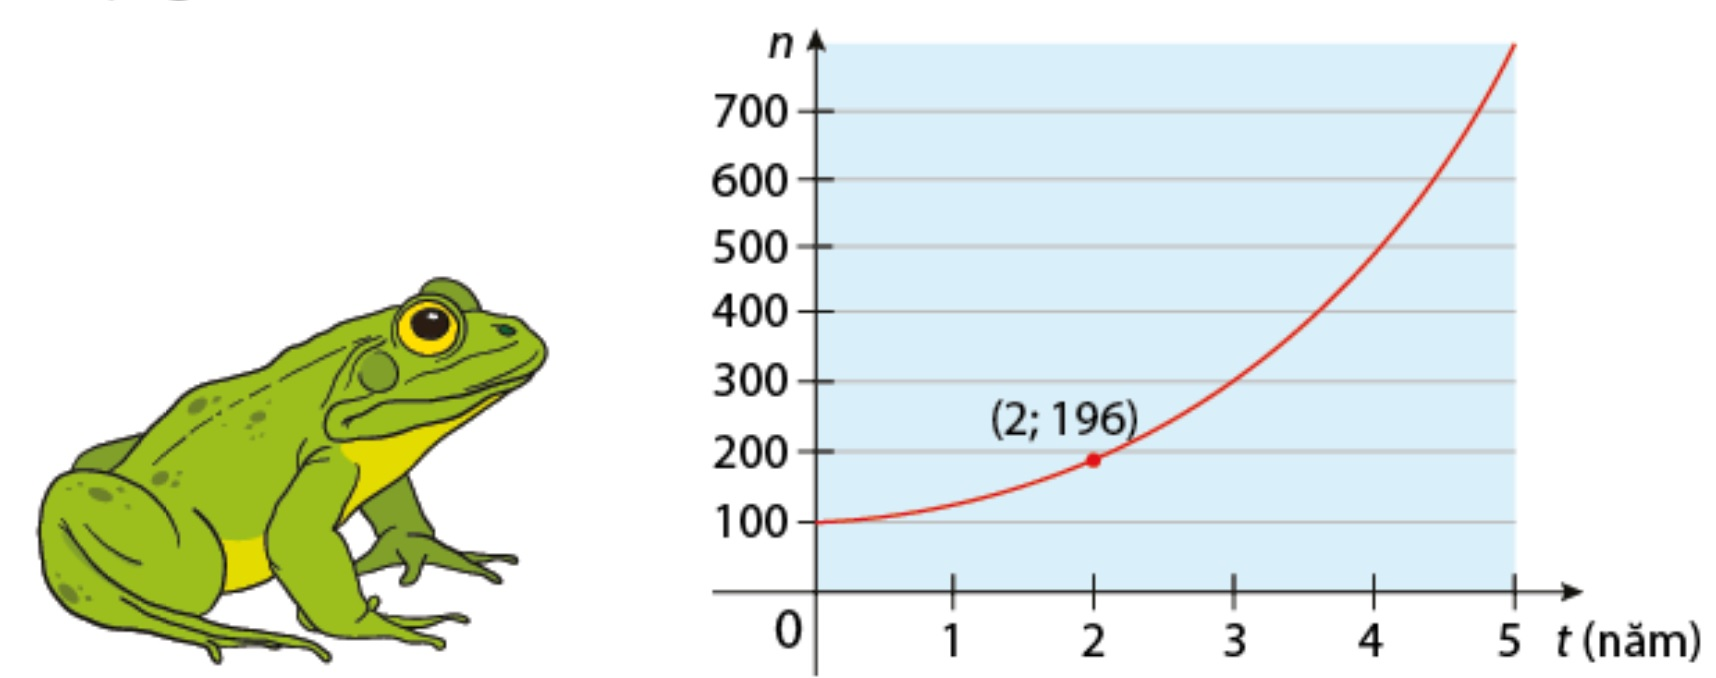
\includegraphics[scale=0.25]{data/11KNTT/data6/h2.jpg}
	\end{center}
	Giả sử số lượng ếch tăng theo hàm số $n(t)=C \cdot a^t$.
	\begin{enumEX}[a)]{1}
		\item Tính số lượng ếch lúc ban đầu.
		\item Tìm hàm số biểu diễn số lượng ếch sau $t$ năm kể từ khi chúng xuất hiện trong ao.
		\item Dự đoán số lượng ếch sau 15 năm.
	\end{enumEX}
	\loigiai{
		\begin{enumerate}[a)]
			\item
			\item
			\item
	\end{enumerate}}
\end{bt} \dongcham{12}

\begin{bt}
	Tìm tất cả giá trị của tham số $m$ để hàm số $y=\ln \left(  x^2-2mx+4 \right)$ có tập xác định là $\mathbb{R}$.
	\loigiai{
		Hàm số đã cho xác định với mọi $x\in \mathbb{R}$ khi và chỉ khi
		\begin{align*}
			&x^2-2m+4>0,\ \forall x\in \mathbb{R} \Leftrightarrow \heva{&1>0\\ &\Delta'<0}\Leftrightarrow m^2-4<0 \Leftrightarrow -2<m<2.
		\end{align*}
	}
\end{bt} \dongcham{12}

\begin{bt}
	Tìm tất cả giá trị của tham số $m$ để hàm số $y=f(x)=\ln (x^2-2mx+m+2)$ có tập xác định là $\mathbb{R}$.
	\loigiai{
		Hàm số $y=f(x)=\ln (x^2-2mx+m+2)$ xác định trên $\mathbb{R}$ khi và chỉ khi \allowdisplaybreaks
		\begin{eqnarray*}
			&&x^2-2mx+m+2>0,\ \forall x\in \mathbb{R}\\
			&\Leftrightarrow&  \heva{&1>0\\&\Delta'=(-m)^2-(m+2)>0}\\
			&\Leftrightarrow&  m^2-m-2>0\\
			&\Leftrightarrow& -1<m<2.
		\end{eqnarray*}
	}
\end{bt} \dongcham{12}

\begin{bt}%[1D4B3-1]
	Tìm tất cả các giá trị của tham số $a$ để hàm số $y=\log_{a^2-2a+1}x$ nghịch biến trên khoảng $(0;+\infty)$.
	\loigiai{		
		Hàm số $y=\log _{a^2-2 a+1} x$ nghịch biến trên khoảng $(0 ;+\infty)$ khi và chỉ khi
		$$
		0<a^2-2 a+1<1 \Leftrightarrow 0<a<2 \,\text{và}\, a \neq 1.
		$$
	}
\end{bt} \dongcham{11}

\begin{bt}%[1K6KJ-4]
	Chu kì bán rã của đồng vị phóng xạ Radi 226 là khoảng $1600$ năm. Giả sử khối lượng $m$ (tính bằng gam) còn lại sau $t$ năm của một lượng Radi 226 được cho bởi công thức:
	$$
	m=25 \cdot\left(\frac{1}{2}\right)^{\tfrac{t}{1600}}
	$$
	\begin{enumerate}[a)]
		\item Khối lượng ban đầu (khi $t=0$) của lượng Radi 226 đó là bao nhiêu?
		\item Sau 2500 năm khối lượng của lượng Radi 226 đó là bao nhiêu?
	\end{enumerate}
	\loigiai{
		\begin{enumerate}[a)]
			\item $m(0)=25 \cdot\left(\frac{1}{2}\right)^{\tfrac{0}{1600}}=25$ g.
			\item $m(2500)=25 \cdot\left(\frac{1}{2}\right)^{\tfrac{2500}{1600}}\approx 8{,}46$ g.
		\end{enumerate}
	}
\end{bt} \dongcham{12}
